\chapter{Introduction}
\label{ch:chap1}


%------------------------------------------
\section{Backgrounds}

\subsection{Engineering Background}

In modern clinic room, the doctors are eagerly looking for a solution which can provide high fidelity and high resolution imaging method to study the peripheral artery disease which is a major cause of amputation in United States. It is prevalent among smokers, diabetics and patient with dyslipidemia. The  current technology can only render two-dimensional,  monochrome and static low-resolution picture. The long waiting time and high expense are two major concerns for all the patients. In recent decades, researchers contribute tremendous effort on improving the diagnosis of stenoses and the quality of imaging\cite{clark1976fluid, nesbitt2009shear, wardlaw2006non, stergiopulos1992computer, long2001numerical}. With the fast development on both hardware and numerical method, the computational simulation can provide 3-D, dynamic, high resolution and fast scan results. Comparing to current CT scan, it's more accurate, faster and cheaper. Moreover, it's also very important that the simulation strategy can bring the doctors and patient that the development of current stenoses and the following consequence after the corresponding treatment. Fig \ref{fig: ch1f1} summarizes some factors which contributing to the interests in computational medical simulation techniques\cite{barry2005features}. Many investigations have been conducted through last decades\cite{feng2012viscous, bertram2010evaluation, nadeem2010simulation, ogulu2005simulation}. However, since this is a fluid-structural interaction problem, both high fidelity fluid and solid solver are needed. 

\begin{figure}[H]
	\centering
	\begin{tabular}{c}
		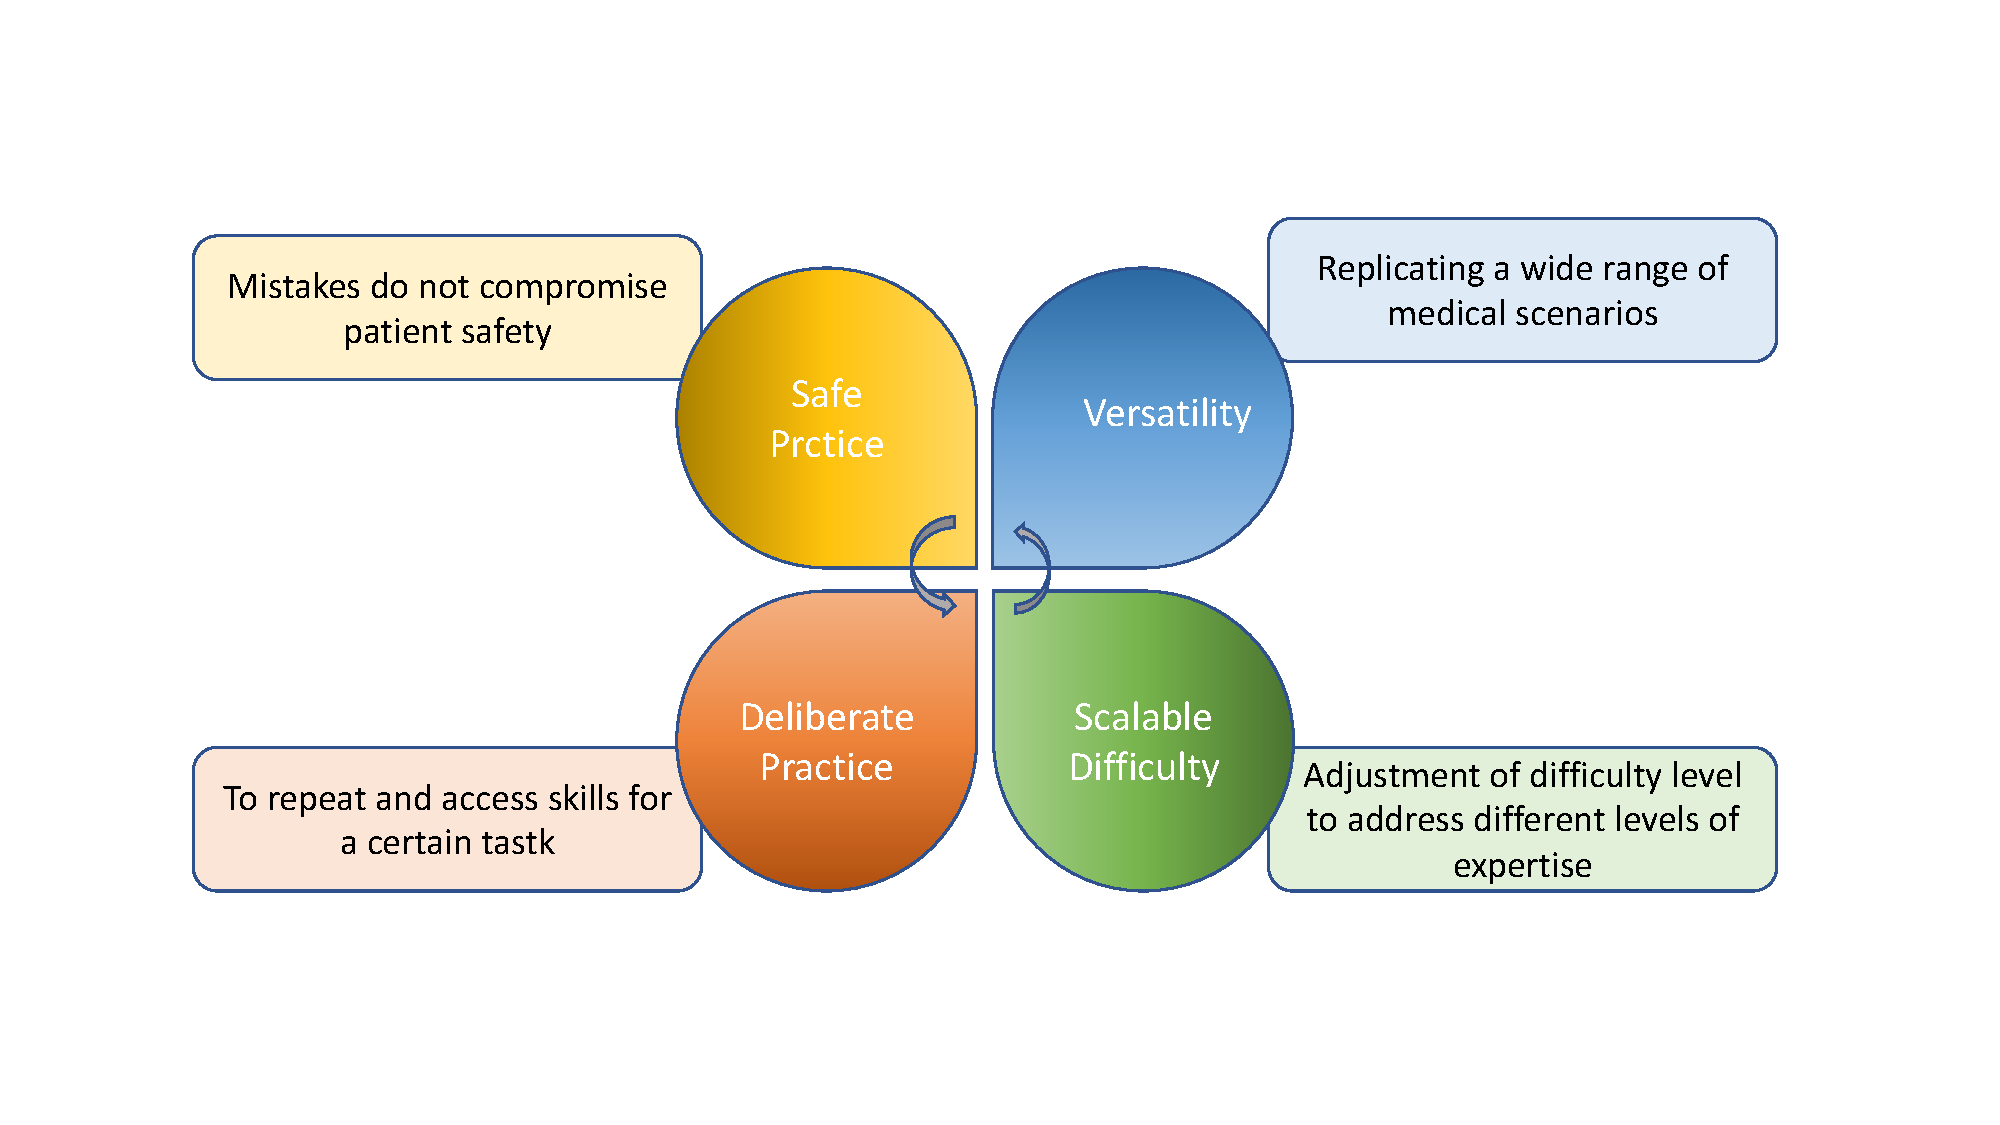
\includegraphics[width=1.0\textwidth]{./pics/computer_simulation}
	\end{tabular}
	\caption{\footnotesize Different factors affecting computer-based medical simulation.} \label{fig: ch1f1}
\end{figure}

The high order parallel fluid solver \cite{liang2007large, liang2007large, liang2009effect} is accomplished and a series of computational fluid dynamics simulation study has been conducted along ideal geometries. To implement the realistic simulation, the tissue of blood vessel shall be considered as elastic material. An accurate and efficient solver for elasticity equation is needed.

\subsection{Numerical Method Review}



%-----------------------------------------------------
\section{Objectives of this Work}
In this work, xxx
